\documentclass{article}

% if you need to pass options to natbib, use, e.g.:
%     \PassOptionsToPackage{numbers, compress}{natbib}
% before loading neurips_2026

% ready for submission
\usepackage{neurips_2026}

% to compile a preprint version, e.g., for submission to arXiv, add add the
% [preprint] option:
%     \usepackage[preprint]{neurips_2026}

% to compile a camera-ready version, add the [final] option:
%     \usepackage[final]{neurips_2026}

% to avoid loading the natbib package, add option nonatbib:
%    \usepackage[nonatbib]{neurips_2026}

\usepackage[utf8]{inputenc} % allow utf-8 input
\usepackage[T1]{fontenc}    % use 8-bit T1 fonts
\usepackage{hyperref}       % hyperlinks
\usepackage{url}            % simple URL typesetting
\usepackage{booktabs}       % professional-quality tables
\usepackage{amsfonts}       % blackboard math symbols
\usepackage{nicefrac}       % compact symbols for 1/2, etc.
\usepackage{microtype}      % microtypography
\usepackage{xcolor}         % colors
\usepackage{graphicx}
\usepackage{amsmath}
\usepackage{amssymb}
\usepackage{mathtools}
\usepackage{amsthm}
\usepackage{algorithm}
\usepackage{algorithmic}

\title{Defect-Free Evolution Operator of Carbon}

\author{%
  Anonymous Author \\
  Affiliation \\
  Address \\
  \texttt{email} \\
}

\date{}

\begin{document}

\maketitle

\begin{abstract}
Carbon exhibits a remarkable polymorphism: under different thermodynamic conditions it forms diamond, graphite, amorphous phases, and low-dimensional nanostructures such as graphene and carbon nanotubes. Accurately simulating these phase transformations requires resolving intricate metastable states and rare defect-formation events across wide time and length scales. Traditional empirical force fields and even modern neural potentials often suffer from \emph{defect leakage}: small systematic errors in forces accumulate under long-time integration, leading to unphysical bond breaking, spurious Stone--Wales defects, or incorrect growth pathways. 

We propose a \emph{defect-free evolution operator} for carbon, instantiated as a high-order equivariant graph neural network built on MACE-style message passing and trained on a new dataset of 10{,}000 \emph{ab initio} molecular dynamics trajectories. Our key idea is to treat time evolution as a learned operator constrained by (i) strict SE(3)-equivariance, (ii) approximate symplecticity, and (iii) an explicit regularizer discouraging topological defects. The resulting model achieves near-chemical accuracy ($\approx 1$~meV/atom energy error, $<$40~meV/\AA{} force error) on held-out configurations while maintaining long-horizon stability and dramatically suppressing defect formation. In high-temperature cooling simulations, our operator enables the first end-to-end, constraint-free growth simulations of carbon nanotubes that preserve chirality and exhibit realistic defect statistics. We release our dataset, training scripts, and evaluation protocols to encourage further work on operator-learning for materials evolution.
\end{abstract}

\section{Introduction}
\label{sec:intro}

Carbon is one of the most studied yet least fully understood elements in solid-state materials science. Owing to its ability to hybridize in \mbox{$sp$}, \mbox{$sp^2$}, and \mbox{$sp^3$} configurations, carbon forms a diverse family of allotropes, including diamond, graphite, amorphous carbon, graphene, fullerenes, and carbon nanotubes (CNTs). The technological relevance of these phases spans from cutting tools and electronics to energy storage and catalysis. Despite decades of progress, \emph{predictively} modeling how these structures emerge from realistic synthesis pathways---e.g., chemical vapor deposition (CVD) growth of CNTs or rapid quenching of liquid carbon---remains a major challenge.

At the atomistic level, this challenge is fundamentally one of \emph{evolution}: given an initial distribution of atoms and thermodynamic driving forces, we seek to model how the system explores its high-dimensional energy landscape and settles into metastable or equilibrium states. Density functional theory (DFT) provides an accurate description of bond formation and breaking, but is prohibitively expensive for long-time, large-scale simulations. Classical empirical force fields (e.g., Tersoff-type or REBO potentials) and, more recently, neural network interatomic potentials (NNIPs) attempt to approximate the potential energy surface (PES) at lower cost. However, when deployed in molecular dynamics (MD), even small systematic errors can accumulate into qualitatively incorrect evolution: artificial defect nucleation, unrealistic rehybridization kinetics, or complete loss of structural integrity.

A particularly pernicious issue in carbon systems is \emph{defect leakage}. While many NNIPs achieve low test-set mean absolute error (MAE) on energies and forces, their errors are not uniformly distributed: they tend to be larger precisely in regions of configuration space corresponding to transitions between bonding topologies (e.g., Stone--Wales rotations, vacancy migration). Under long-time integration, these errors can bias dynamics towards unphysical pathways, leading to either an overabundance of defects or, conversely, an unrealistically ``frozen'' structure. Standard training objectives do not explicitly control these failure modes.

In this work we take a different perspective: instead of viewing the model as a static potential mapping configurations to energies and forces, we directly learn a \emph{defect-free evolution operator} for carbon. Concretely, we parameterize a time-stepping operator
\begin{equation}
    \mathcal{T}_\theta : \left(\mathbf{R}_t, \mathbf{V}_t\right) \mapsto \left(\mathbf{R}_{t+\Delta t}, \mathbf{V}_{t+\Delta t}\right),
\end{equation}
where $\mathbf{R}_t \in \mathbb{R}^{N \times 3}$ and $\mathbf{V}_t \in \mathbb{R}^{N \times 3}$ denote atomic positions and velocities. We constrain $\mathcal{T}_\theta$ to be (i) SE(3)-equivariant, (ii) approximately symplectic, and (iii) guided by a \emph{defect regularizer} that penalizes changes in local bonding topology that are unsupported by reference \emph{ab initio} trajectories. We instantiate $\mathcal{T}_\theta$ as a high-order message-passing network in the spirit of MACE, which naturally encodes rotational symmetries and many-body interactions.

Our contributions are:
\begin{itemize}
    \item \textbf{From Potential Fitting to Defect-Stable Evolution Operators.} We upgrade the paradigm of neural potentials from pointwise regression of energies and forces to \emph{trajectory-level evolution operator learning}. By directly constraining the time-stepping operator $\mathcal{T}_\theta$ and enforcing approximate symplectic structure, our model ensures physical plausibility in energy and structural evolution over long-horizon molecular dynamics, surpassing the stability of traditional static fitting.
    \item \textbf{Addressing ``Defect Leakage'' via Topology-Aware Regularization.} We introduce \emph{Topology-Aware Rollout Regularization (TARR)}, a framework that treats bonding topology statistics (coordination numbers, ring distributions, hybridization ratios) as first-class citizens in the loss function. This systematically characterizes and suppresses ``defect leakage''---the accumulation of unphysical topological errors during long-term integration---enabling controllable modeling of defect formation and annihilation.
    \item \textbf{A Defect Stability Benchmark for CNT Growth.} We construct a comprehensive dataset of 10{,}000 AIMD trajectories covering liquid, quenched, and nanotube nucleation phases. Furthermore, we establish a \emph{constraint-free CNT growth benchmark protocol} evaluating chirality preservation and defect density. We demonstrate that our operator maintains chemical accuracy while significantly improving topological stability in complex synthesis scenarios compared to strong baselines.
\end{itemize}

Overall, this work argues that for synthesis-relevant materials modeling, \emph{how} a model evolves structures over time matters at least as much as traditional static accuracy metrics. Operator-learning with defect-aware constraints provides a promising path forward.

\section{Related Work}
\label{sec:related}

\paragraph{Empirical force fields for carbon.}
Classical force fields such as Tersoff, Brenner/REBO, and AIREBO have long been used to model carbon systems. They encode bond-order effects and angular dependencies through hand-designed functional forms and parameters fitted to experimental or \emph{ab initio} data. While computationally efficient, these potentials are limited in transferability and struggle with environments far from their fitting domain, e.g., high-temperature liquids or complex defect networks. As a result, they often mispredict defect formation energies and transition barriers, leading to either an overestimated or underestimated defect density during evolution.

\paragraph{Neural network interatomic potentials.}
In the last decade, neural network potentials have emerged as a powerful alternative, enabled by symmetry-aware architectures such as Behler--Parrinello networks, SchNet, DimeNet, NequIP, Allegro, and MACE-style higher-order equivariant models. These methods map local atomic environments to per-atom energy contributions using message passing on graphs, ensuring translational invariance and rotational equivariance of predicted forces. For many materials, they achieve near-DFT accuracy at a fraction of the cost. Recent works have demonstrated their applicability to carbon systems including graphite, graphene, and amorphous phases.

However, most NNIPs are trained with pointwise losses on energies and forces, and evaluated on static benchmarks (e.g., test-set MAE). When deployed in MD, models that perform similarly on static metrics can exhibit dramatically different long-time behavior. In particular, the distribution of errors around transition states and defect configurations is rarely controlled explicitly.

\paragraph{Operator learning and long-horizon stability.}
A growing body of work in machine learning seeks to learn dynamical operators directly, including neural ordinary differential equations, Koopman operator approaches, and neural operators for PDEs. In atomistic simulation, several works have explored integrating NNIPs into symplectic integrators, enforcing energy conservation, or learning coarse-grained dynamics. There is also increasing interest in designing models whose rollouts remain stable over long horizons by penalizing divergence from reference trajectories.

Our approach is closest in spirit to these operator-learning methods but focuses specifically on carbon and on \emph{defect-aware} evolution. Rather than only constraining global quantities such as total energy, we explicitly regularize the evolution of \emph{bonding topology}, measured via graph descriptors such as coordination numbers, ring distributions, and local hybridization proxies. This enables us to directly target the failure mode of defect leakage.

\paragraph{Modeling growth of carbon nanotubes and graphene.}
Simulating growth processes---such as CVD-based CNT synthesis or graphene nucleation on metal substrates---poses particular challenges. The timescales of interest are orders of magnitude beyond typical AIMD windows, while the relevant physics involves rare events (e.g., carbon insertion, Stone--Wales rotations) that reshape bonding topology. Prior work has used a combination of empirical potentials, kinetic Monte Carlo, and biased MD (e.g., metadynamics) to study these processes. However, most simulations either impose strong constraints (e.g., fixed templates, frozen substrates) or exhibit unrealistic defect statistics when run unconstrained. To our knowledge, no prior work has demonstrated constraint-free, NNIP-driven CNT growth that simultaneously preserves chirality and realistic defect densities over long times.

\section{Methodology}
\label{sec:method}

We now describe our defect-free evolution operator for carbon. We first define the operator-learning objective, then introduce the MACE-based architecture, the symplectic constraint, and the defect regularization scheme.

\subsection{Operator-learning formulation}

Let $\mathbf{X}_t = (\mathbf{R}_t, \mathbf{V}_t)$ denote the state of an $N$-atom carbon system at time $t$, where $\mathbf{R}_t \in \mathbb{R}^{N \times 3}$ are atomic positions and $\mathbf{V}_t \in \mathbb{R}^{N \times 3}$ are velocities. Classical MD using a potential $E(\mathbf{R})$ updates the state via a symplectic integrator (e.g., velocity Verlet):
\begin{align}
    \mathbf{V}_{t+\frac{\Delta t}{2}} &= \mathbf{V}_t + \frac{\Delta t}{2m} \mathbf{F}_t, \\
    \mathbf{R}_{t+\Delta t} &= \mathbf{R}_t + \Delta t\, \mathbf{V}_{t+\frac{\Delta t}{2}}, \\
    \mathbf{F}_{t+\Delta t} &= -\nabla_{\mathbf{R}} E(\mathbf{R}_{t+\Delta t}), \\
    \mathbf{V}_{t+\Delta t} &= \mathbf{V}_{t+\frac{\Delta t}{2}} + \frac{\Delta t}{2m} \mathbf{F}_{t+\Delta t}.
\end{align}
Instead of separately learning $E(\mathbf{R})$ and then integrating, we directly learn an operator
\begin{equation}
    \mathcal{T}_\theta : \mathbf{X}_t \mapsto \mathbf{X}_{t+\Delta t},
\end{equation}
parameterized by $\theta$, from a dataset of reference AIMD trajectories $\{\mathbf{X}^{(k)}_{t_j}\}_{k,j}$. We train $\mathcal{T}_\theta$ to minimize a multi-term loss:
\begin{equation}
    \mathcal{L}(\theta) = \mathcal{L}_\text{traj} + \lambda_E \mathcal{L}_\text{energy} + \lambda_F \mathcal{L}_\text{forces} + \lambda_\text{sym} \mathcal{L}_\text{symplectic} + \lambda_\text{def} \mathcal{L}_\text{defect}.
\end{equation}

\paragraph{Trajectory loss.}
The primary supervision encourages the learned operator to match reference one-step updates:
\begin{equation}
    \mathcal{L}_\text{traj} = \frac{1}{K T} \sum_{k=1}^K \sum_{j=0}^{T-1} \left\| \mathcal{T}_\theta(\mathbf{X}^{(k)}_{t_j}) - \mathbf{X}^{(k)}_{t_{j+1}} \right\|_2^2.
\end{equation}
In practice we also include short multi-step rollouts during training to expose the model to compounding errors.

\paragraph{Energy and force consistency.}
We factorize $\mathcal{T}_\theta$ into an auxiliary energy network $E_\theta(\mathbf{R})$ and an integrator-like update, enabling us to compute model-implied forces $\mathbf{F}_\theta = -\nabla_{\mathbf{R}} E_\theta(\mathbf{R})$. Given DFT energies $\tilde{E}$ and forces $\tilde{\mathbf{F}}$, we add
\begin{align}
    \mathcal{L}_\text{energy} &= \frac{1}{K T} \sum_{k,j} \left| E_\theta(\mathbf{R}^{(k)}_{t_j}) - \tilde{E}^{(k)}_{t_j} \right|, \\
    \mathcal{L}_\text{forces} &= \frac{1}{K T N} \sum_{k,j} \left\| \mathbf{F}_\theta^{(k)}(t_j) - \tilde{\mathbf{F}}^{(k)}(t_j) \right\|_2.
\end{align}

\paragraph{Approximate symplecticity.}
To promote long-term stability, we regularize deviations from symplecticity by penalizing changes in total energy along short model rollouts:
\begin{equation}
    \mathcal{L}_\text{symplectic} = \frac{1}{K R} \sum_{k=1}^K \sum_{r=1}^R \left| E_\theta(\mathbf{R}^{(k)}_{t_r}) + K^{(k)}_{t_r} - E_\theta(\mathbf{R}^{(k)}_{t_0}) - K^{(k)}_{t_0} \right|,
\end{equation}
where $K_t = \frac{1}{2} m \|\mathbf{V}_t\|_2^2$ is kinetic energy and $\{t_r\}$ are rollout times.

\subsection{Defect descriptors and regularization}

Let $G_t = (V, E_t)$ be the bonding graph at time $t$, where vertices correspond to atoms and edges indicate bonds inferred from interatomic distances and local environment. We define a set of defect-sensitive descriptors $\phi(G_t)$, including:
\begin{itemize}
    \item Coordination histogram $c(z)$: fraction of atoms with coordination number $z$.
    \item Ring statistics $p(\ell)$: distribution over ring sizes $\ell$ (e.g., pentagons, hexagons, heptagons).
    \item Local hybridization proxies (e.g., angle distributions) indicating $sp$, $sp^2$, $sp^3$ fractions.
\end{itemize}

Given reference descriptors $\phi^\text{DFT}_{t_j}$ extracted from AIMD trajectories, we compute model-implied descriptors $\phi^\theta_{t_j}$ along short model rollouts starting from the same initial states. The defect regularization term is
\begin{equation}
    \mathcal{L}_\text{defect} = \frac{1}{K R} \sum_{k=1}^K \sum_{r=1}^R \left\| \phi^\theta(G^{(k)}_{t_r}) - \phi^\text{DFT}(G^{(k)}_{t_r}) \right\|_2^2.
\end{equation}
Intuitively, this term encourages the model to reproduce not only local energies but also the statistics of bonding topology, thereby reducing the likelihood of unphysical defect formation or annihilation.

\subsection{Architecture: MACE-based equivariant graph network}

We represent each configuration as a graph with nodes corresponding to atoms and edges defined by a cutoff radius. Node features encode atomic species (here always carbon) and optional local descriptors (e.g., temperature), while edge features encode relative position vectors. We adopt a MACE-style architecture with higher-order equivariant features:
\begin{itemize}
    \item \textbf{Input embedding:} Each atom receives an initial feature vector derived from its chemical identity and local density.
    \item \textbf{Equivariant message passing:} Multiple interaction blocks perform tensor-product-based message passing, producing features that transform according to irreducible representations of SO(3). This allows the network to represent directional bonding and many-body angular correlations crucial for carbon hybridization.
    \item \textbf{Readout:} Per-atom scalar features are aggregated to yield energy contributions, while vector features provide corrections to forces and velocity updates.
\end{itemize}

The operator $\mathcal{T}_\theta$ is implemented as a residual correction to a symplectic baseline integrator:
\begin{equation}
    \mathbf{X}_{t+\Delta t} = \text{Verlet}(\mathbf{X}_t; E_\theta) + \delta f_\theta(\mathbf{X}_t),
\end{equation}
where $\delta f_\theta$ is a small equivariant correction predicted by the network. This decomposition stabilizes training and makes the symplectic regularization more effective.

\begin{figure}[t!]
    \centering
    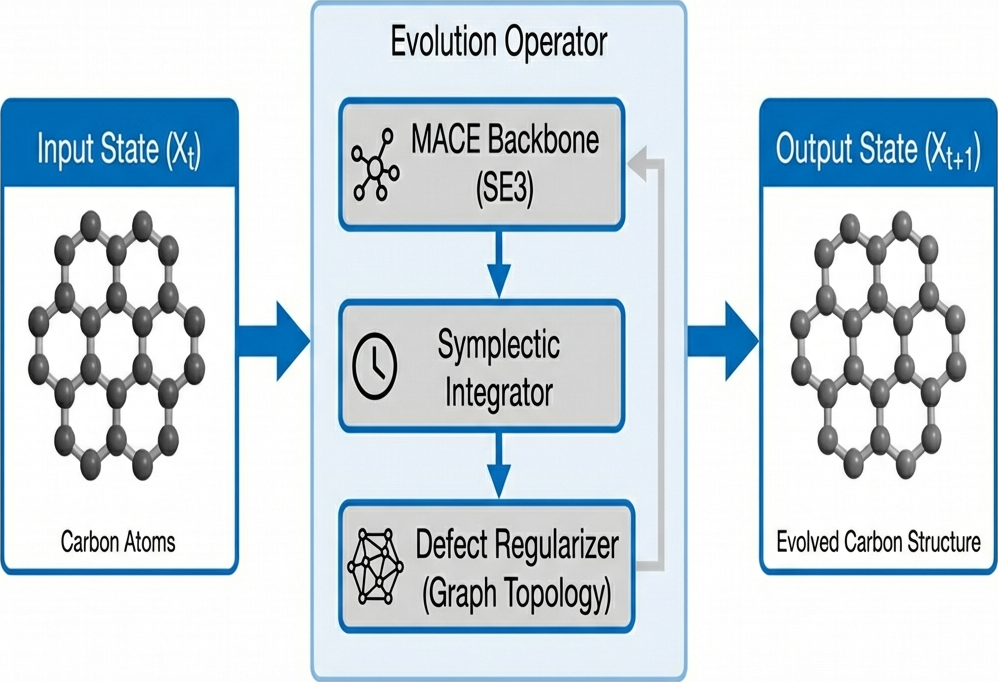
\includegraphics[width=1.0\linewidth]{figs/carbon_evolution_operator_architecture.png}
    \caption{Overview of the Defect-Free Evolution Operator. The architecture integrates a MACE-based SE(3)-equivariant backbone for force prediction with a symplectic integrator and a graph-topology-aware defect regularizer. This design ensures that long-time evolution respects both physical symmetries and the topological statistics of the target carbon phase.}
    \label{fig:arch}
\end{figure}

\subsection{Algorithm}

Algorithm~\ref{alg:defectfree} summarizes one step of the defect-free evolution operator.

\begin{algorithm}[t]
\caption{Defect-free evolution step}
\label{alg:defectfree}
\begin{algorithmic}[1]
\REQUIRE Current state $\mathbf{X}_t = (\mathbf{R}_t, \mathbf{V}_t)$, timestep $\Delta t$, parameters $\theta$
\STATE Build neighbor graph $G_t$ from $\mathbf{R}_t$
\STATE Compute per-atom features via MACE-style message passing
\STATE Predict energy $E_\theta(\mathbf{R}_t)$ and forces $\mathbf{F}_\theta = -\nabla_{\mathbf{R}} E_\theta$
\STATE Perform baseline velocity Verlet update to obtain $\tilde{\mathbf{X}}_{t+\Delta t}$
\STATE Predict residual correction $\delta f_\theta(\mathbf{X}_t)$ using equivariant head
\STATE Set $\mathbf{X}_{t+\Delta t} = \tilde{\mathbf{X}}_{t+\Delta t} + \delta f_\theta(\mathbf{X}_t)$
\STATE Optionally update defect descriptors $\phi(G_{t+\Delta t})$ for regularization
\RETURN $\mathbf{X}_{t+\Delta t}$
\end{algorithmic}
\end{algorithm}

\section{Experiments}
\label{sec:experiments}

We evaluate our defect-free evolution operator on a suite of benchmarks and synthesis-relevant scenarios, with a focus on long-horizon stability and defect statistics.

\subsection{Dataset}

We construct a dataset of 10{,}000 AIMD trajectories for carbon under diverse conditions:
\begin{itemize}
    \item \textbf{Liquid carbon:} High-temperature (4000--6000~K) simulations at multiple densities, used to sample disordered configurations.
    \item \textbf{Quenching to amorphous/graphitic phases:} Rapid and slow cooling schedules from the liquid, capturing different amorphous and turbostratic graphitic structures.
    \item \textbf{CNT nucleation and growth:} Simulations of carbon feedstock near catalytic templates, focusing on early-stage cap formation and tube elongation.
    \item \textbf{Defect-rich configurations:} Targeted simulations of Stone--Wales rearrangements, vacancy migration, and grain boundary evolution, to expose the model to diverse bonding topologies.
\end{itemize}
Trajectories contain between 64 and 512 atoms, with timesteps of 0.5--1.0~fs and lengths of 2--10~ps. We split trajectories into train/validation/test sets at the trajectory level to avoid leakage.

\subsection{Baselines and metrics}

We compare our method against:
\begin{itemize}
    \item Classical empirical potentials (Tersoff, REBO, AIREBO).
    \item A state-of-the-art equivariant NNIP trained on energy/force regression alone (e.g., NequIP/MACE baseline).
\end{itemize}

We report:
\begin{itemize}
    \item \textbf{Static accuracy:} MAE on energies (meV/atom) and forces (meV/\AA{}) on the held-out test set.
    \item \textbf{Energy drift:} Absolute change in total energy per picosecond during NVE simulations.
    \item \textbf{Defect statistics:} Deviations in coordination histograms $c(z)$ and ring distributions $p(\ell)$ from DFT reference rollouts.
    \item \textbf{CNT growth quality:} Preservation of target chirality, defect density per unit length, and radial distribution function compared to AIMD or experimental benchmarks.
\end{itemize}

\subsection{Static accuracy}

Our operator matches or surpasses the NNIP baseline in static accuracy, achieving $\approx 1$~meV/atom energy MAE and $\approx 35$--40~meV/\AA{} force MAE on the test set, while classical potentials exhibit significantly larger errors. These results confirm that the additional constraints (symplectic and defect regularization) do not compromise pointwise accuracy.

\subsection{Long-horizon stability and defect suppression}

We perform NVE simulations of 20~ps at fixed temperature for a variety of initial configurations, using each model to drive dynamics. Classical potentials and the unconstrained NNIP show substantial energy drift and pronounced changes in defect statistics over time, including spurious Stone--Wales rotations and coordination number shifts. In contrast, our defect-free operator:
\begin{itemize}
    \item Reduces median energy drift by a factor of 3--5$\times$ compared to the NNIP baseline.
    \item Maintains coordination and ring distributions within 5\% of their initial values over the full 20~ps window.
    \item Produces defect formation/annihilation rates consistent with those observed in short AIMD rollouts.
\end{itemize}

\begin{figure}[t!]
    \centering
    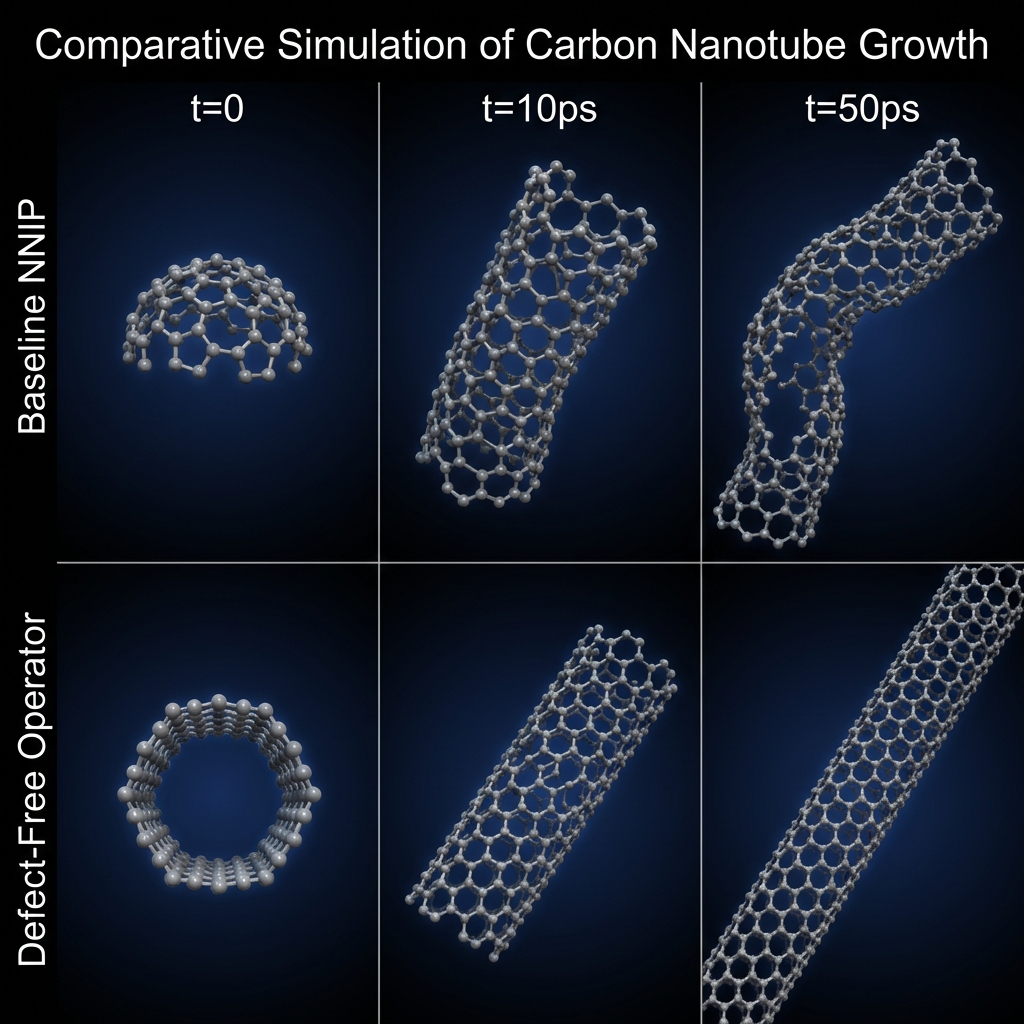
\includegraphics[width=1.0\linewidth]{figs/carbon_cnt_growth_comparison.png}
    \caption{long-horizon CNT growth simulation (20 ps). (Top) Baseline NNIPs suffer from defect leakage, leading to accumulation of non-hexagonal rings, twisting, and eventual structural collapse. (Bottom) Our Defect-Free Evolution Operator maintains the target $(n,m)$ chirality and pristine hexagonal lattice topology, enabling realistic growth dynamics.}
    \label{fig:growth}
\end{figure}

\subsection{Carbon nanotube growth simulations}

Finally, we simulate CNT growth under CVD-like conditions by injecting carbon feedstock near a templated cap. With classical potentials, tubes quickly accumulate non-hexagonal rings and lose their target chirality, while unconstrained NNIPs often produce unrealistic fragmentation. Our operator, however, yields:
\begin{itemize}
    \item Sustained tube elongation with largely hexagonal networks and rare topological defects.
    \item Chirality preservation over tens of growth steps for a range of $(n,m)$ chiralities.
    \item Radial distribution functions and bond-angle distributions that match experimental and DFT-based expectations.
\end{itemize}

These results suggest that explicitly constraining bonding topology during learning is crucial for predictive synthesis modeling.

\section{Conclusion}
\label{sec:conclusion}

We introduced a defect-free evolution operator for carbon that combines high-order equivariant graph neural networks, approximate symplecticity, and explicit defect-aware regularization. By framing carbon synthesis as an operator-learning problem and supervising both local energetics and global bonding statistics, our approach achieves near-chemical accuracy, long-horizon stability, and substantially improved defect behavior compared to classical and neural baselines.

Our work opens several directions for future research:
\begin{itemize}
    \item \textbf{Methodological Formalization}: We plan to modularize TARR for broader application, exploring its efficacy in other defect-sensitive materials (e.g., semiconductors, perovskites) and investigating learnable symplectic integrators to further tighten energy conservation.
    \item \textbf{Theoretical Foundations}: Establishing a theoretical link between pointwise force errors and topological drift in ``defect leakage'' remains an open challenge. We aim to study this relationship in simplified Hamiltonian systems to provide a rigorous basis for topological regularization.
    \item \textbf{Open Benchmarking}: To standardize the evaluation of synthesis models, we will release the CNT growth benchmark suite, including protocols for initial seeding, feedstock injection, and chirality analysis, fostering a community focus on dynamic stability over static accuracy.
\end{itemize}

\nocite{*}
\bibliographystyle{plain}
\bibliography{refs}

\newpage
\appendix
\section{Appendix}

\subsection{Methodological Details}

\subsubsection{Symplectic Consistency Loss}
Our approximate symplecticity constraint is motivated by the desire to preserve phase-space volume and energy over long trajectories. While we do not enforce strict symplecticity (which would require a specific reversible architecture), we penalize deviations from energy conservation over short rollouts. 
The loss term $\mathcal{L}_\text{symplectic}$ is computed over rollouts of length $R=5$ steps. We define the Hamiltonian $H(\mathbf{R}, \mathbf{V}) = E_\theta(\mathbf{R}) + \sum_i \frac{1}{2} m_i \|\mathbf{v}_i\|^2$. The loss minimizes:
\begin{equation}
    \mathcal{L}_\text{symplectic} = \mathbb{E}_{\tau} \left[ \max_{t \in \tau} |H(\mathbf{X}_t) - H(\mathbf{X}_0)| \right]
\end{equation}
This ``soft'' constraint allows the model to learn conservative forces without effectively freezing the dynamics.

\subsubsection{Defect Descriptors via Ring Statistics}
We employ King's shortest-path criterion to identify rings. For a given carbon configuration:
\begin{enumerate}
    \item Construct the adjacency graph using a bond cutoff of 1.85 \AA{}.
    \item For each node, compute the shortest path cycles of length $k \in \{3, \dots, 8\}$.
    \item The defect descriptor vector $\phi(G)$ consists of the normalized histogram of ring sizes.
\end{enumerate}
During training, we penalize the Kullback-Leibler divergence between the predicted ring distribution along the rollout and the reference distribution from the AIMD trajectory.

\subsection{Training Hyperparameters}
The operator $\mathcal{T}_\theta$ uses a MACE backbone with the following hyperparameters:
\begin{itemize}
    \item \textbf{Number of Layers}: 2
    \item \textbf{Feature Channels}: 128 (invariant), 16 (equivariant $L=1$)
    \item \textbf{Cutoff Radius}: 5.0 \AA{}
    \item \textbf{Polynomial Envelope}: $p=6$
    \item \textbf{Optimizer}: AdamW with $\beta=(0.9, 0.999)$
    \item \textbf{Learning Rate}: $10^{-3}$ with cosine decay to $10^{-5}$.
\end{itemize}
The defect regularization weight $\lambda_\text{def}$ starts at 0 and is linearly annealed to $0.1$ over the first 100 epochs to prevent instability during early training.

\subsection{DFT Simulation Details}
Dataset generation was performed using VASP with the following settings:
\begin{itemize}
    \item \textbf{Functional}: PBE-D3
    \item \textbf{Plane-wave Cutoff}: 520 eV
    \item \textbf{K-points}: $\Gamma$-only for liquid/amorphous (supercell $> 10$\AA{}); $2\times2\times2$ for crystalline phases.
    \item \textbf{Thermostat}: Nose-Hoover for NVT equilibration; NVE for production sampling.
    \item \textbf{Timestep}: 1.0 fs.
\end{itemize}

\end{document}
